\documentclass[english,10pt,aspectratio=169]{beamer}

\usepackage{amsmath}
\usepackage{array}
\usepackage[T1]{fontenc}
\usepackage{listings}
\usepackage{tikz}
\usepackage{ulem}

%%%%%%%%%%%%%%%%%%%%%%%%%%%%%%%%%%%%%%%%%%%%%%%%%%%%%%%%%%%
% beamer
%%%%%%%%%%%%%%%%%%%%%%%%%%%%%%%%%%%%%%%%%%%%%%%%%%%%%%%%%%%
\mode<presentation>
\usetheme{singapore}
\usecolortheme{orchid}

%%%%%%%%%%%%%%%%%%%%%%%%%%%%%%%%%%%%%%%%%%%%%%%%%%%%%%%%%%%
% listings
%%%%%%%%%%%%%%%%%%%%%%%%%%%%%%%%%%%%%%%%%%%%%%%%%%%%%%%%%%%
\lstdefinestyle{PythonStyle}{
	basicstyle=\scriptsize\ttfamily,
	language=Python,
	numbers=left,
	tabsize=4
}
\lstset{basicstyle=\small,style=PythonStyle}

%%%%%%%%%%%%%%%%%%%%%%%%%%%%%%%%%%%%%%%%%%%%%%%%%%%%%%%%%%%
% tikz
%%%%%%%%%%%%%%%%%%%%%%%%%%%%%%%%%%%%%%%%%%%%%%%%%%%%%%%%%%%
\usetikzlibrary{shapes.geometric, arrows}
\tikzstyle{startstop} = [
	rectangle,
	rounded corners,
	minimum width=1cm,
	minimum height=0.5cm,
	text centered,
	draw=black,
	fill=red!30
]
\tikzstyle{io} = [
	trapezium,
	trapezium left angle=70,
	trapezium right angle=110,
	minimum width=1cm,
	minimum height=0.5cm,
	text centered,
	draw=black,
	fill=blue!30
]
\tikzstyle{process} = [
	rectangle,
	minimum width=1cm,
	minimum height=0.5cm,
	text centered,
	draw=black,
	fill=orange!30
]
\tikzstyle{decision} = [
	diamond,
	minimum width=1cm,
	minimum height=0.5cm,
	text centered,
	draw=black,
	fill=green!30
]
\tikzstyle{arrow} = [thick, ->, >=stealth]
%%%%%%%%%%%%%%%%%%%%%%%%%%%%%%%%%%%%%%%%%%%%%%%%%%%%%%%%%%%
% commands
%%%%%%%%%%%%%%%%%%%%%%%%%%%%%%%%%%%%%%%%%%%%%%%%%%%%%%%%%%%
\newcommand{\focus}[1]{\textcolor{blue}{#1}}

\newcommand{\hideit}[1]{%
  \only<0| handout:1>{\mbox{}}%
  \invisible<0| handout:1>{#1}%
}

\def\presentationtitle{\textbf{
	Spending less time bug fixing by \\
	spending more time unit testing
}}

\title{\large\presentationtitle}
\author{\textbf{
	<Name>
}}
\date{}

\begin{document}

%%%%%%%%%%%%%%%%%%%%%%%%%%%%%%%%%%%%%%%%%%%%%%%%%%%%%%%%%%%
% code listings 
%%%%%%%%%%%%%%%%%%%%%%%%%%%%%%%%%%%%%%%%%%%%%%%%%%%%%%%%%%%
\defverbatim[colored]\coveragecode{%
\begin{lstlisting}[linewidth=0.5\textwidth]
def is_fizzbuzz(num: int) -> bool:
    if num % 3 and num % 5:
        return True
    return some_var

def test_fizzbuzz():
    result = is_fizzbuzz(3)
    assert result
\end{lstlisting}
}

\defverbatim[colored]\coveragecodetwo{%
\begin{lstlisting}[linewidth=0.5\textwidth]
def is_fizzbuzz(num: int) -> bool:
    return True if num % 3 and num % 5 else some_var

def test_fizzbuzz():
    result = is_fizzbuzz(3)
    assert result
\end{lstlisting}
}

\defverbatim[colored]\coveragecodebranch{%
\begin{lstlisting}[linewidth=0.5\textwidth]
def generate_number(
    cond_1: bool = True,
    cond_2: bool = True,
    cond_3: bool = True,
) -> int:
    if cond_1:
        num = 1
    if cond_2:
        num = 2
    if cond_3:
        num = 3
    return num
\end{lstlisting}
}


\begin{frame}
	\titlepage
\end{frame}

% To begin with a quote from the author, "There's much more to unit testing than
% the act of writing tests." Hopefully this presentation will be able to get you
% to think more about how to craft unit tests.
\begin{frame}
	\begin{quote}
		There's much more to unit testing than the act of writing tests.
		\begin{flushright}
			\tiny{---Khorikov, \textup{Unit Testing Principles, Practices, and Patterns}, 3}
		\end{flushright}
	\end{quote}
\end{frame}

% The goal of unit testing is to enable sustainable growth of the software
% project. The figure below show the growth dynamics of a typical project without
% tests. You start off quick, completing user stories after user stories, without
% having to "waste" writing these pesky tests.
% But eventually progress slows to a halt, the code base has grown complex and
% disorganized, fixing one bug introduces several others, and changing one part
% of the software breaks several others. And it's hard to bring it back to
% stability.
% This is where tests help, they help detect regressions and ensure existing
% functionalities work even after refactoring or introducing new features.
\begin{frame}{The goal of unit testing}
	To enable \textbf{sustainable} growth of software project.
	\begin{columns}[T]
		\begin{column}{0.5\textwidth}
			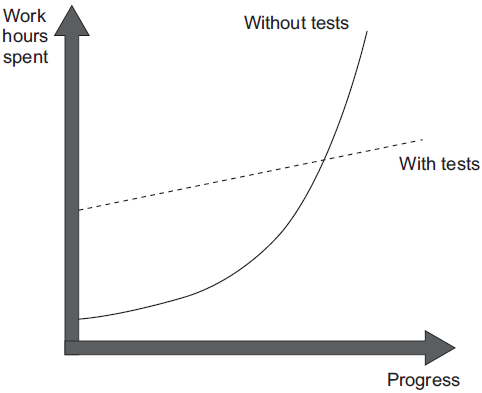
\includegraphics[width=\textwidth]{images/vs_no_test.png}
		\end{column}
		\begin{column}{0.5\textwidth}
		\end{column}
	\end{columns}
\end{frame}

% But it's not enough to just write tests. Badly written tests still result in
% the same picture. They help slow down the initial decline in development speed
% but doesn't really change much overall. Before we look at what makes a good unit
% test, let's first look at code coverage metrics which can help you gauge if you
% are testing enough.
\begin{frame}{The goal of unit testing}
	To enable \textbf{sustainable} growth of software project.
	\begin{columns}[T]
		\begin{column}{0.5\textwidth}
			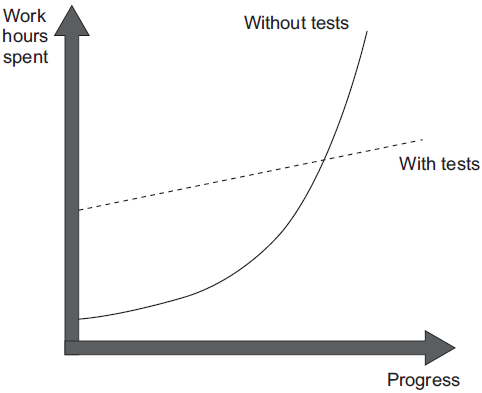
\includegraphics[width=\textwidth]{images/vs_no_test.png}
		\end{column}
		\begin{column}{0.5\textwidth}
			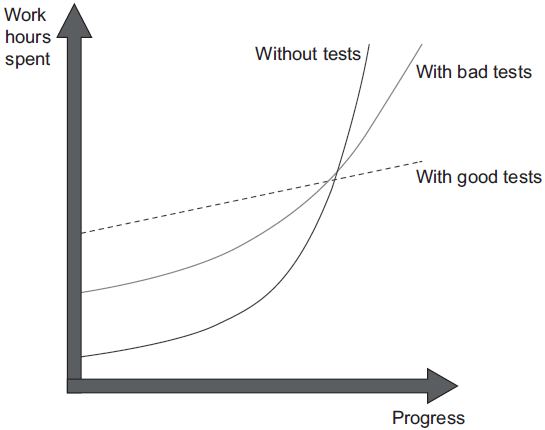
\includegraphics[width=\textwidth]{images/vs_bad_test.png}
		\end{column}
	\end{columns}
\end{frame}

% The common belief is that the higher the coverage number, the better the test
% suite. Unfortunately, it's not that simple. While 10% is a good indication
% that you aren't testing enough, 100% coverage doesn't guarantee you have a
% good quality test suite. We take a look at a few coverage metrics to see why
% this is so.
% We will discuss 4 types of coverage metrics. Path and condition coverage are
% struck out because while they're nice to think about, they're impractical to
% actually implement.
% < describe the code and coverage stats > 
\begin{frame}{Coverage metrics}
	\focus{Statement} vs Branch vs \sout{Path} vs \sout{Condition}
	\begin{columns}[T]
		\begin{column}[]{0.6\textwidth}
			\begin{minipage}{\linewidth}
				\coveragecode
			\end{minipage}
		\end{column}
		\begin{column}[]{0.4\textwidth}
			\begin{flalign*}
				&\frac{Number\ of\ statements\ executed}{Total\ number\ of\ statements}\\
				\approx\ &67 \%
			\end{flalign*}
		\end{column}
	\end{columns}
\end{frame}

\begin{frame}{Coverage metrics}
	\focus{Statement} vs Branch vs \sout{Path} vs \sout{Condition}
	\begin{columns}[T]
		\begin{column}[]{0.6\textwidth}
			\begin{minipage}{\linewidth}
				\coveragecodetwo
			\end{minipage}
		\end{column}
		\begin{column}[]{0.4\textwidth}
			\begin{flalign*}
				&\frac{Number\ of\ statements\ executed}{Total\ number\ of\ statements}\\
				=\ &100 \%
			\end{flalign*}
		\end{column}
	\end{columns}
\end{frame}

\begin{frame}{Coverage metrics}
	Statement vs \focus{Branch} vs \sout{Path} vs \sout{Condition}
	\begin{columns}[T]
		\begin{column}[]{0.6\textwidth}
			\begin{minipage}{\linewidth}
				\coveragecodetwo
			\end{minipage}
		\end{column}
		\begin{column}[]{0.4\textwidth}
			\begin{flalign*}
				&\frac{Branches\ traversed}{Total\ number\ of\ branches}\\
				=\ &50 \%
			\end{flalign*}
		\end{column}
	\end{columns}
\end{frame}

\begin{frame}{Coverage metrics}
	Statement vs \focus{Branch} vs \sout{Path} vs \sout{Condition}
	\begin{columns}[T]
		\begin{column}[]{0.6\textwidth}
			\begin{minipage}{\linewidth}
				\coveragecodetwo
			\end{minipage}
		\end{column}
		\begin{column}[]{0.4\textwidth}
			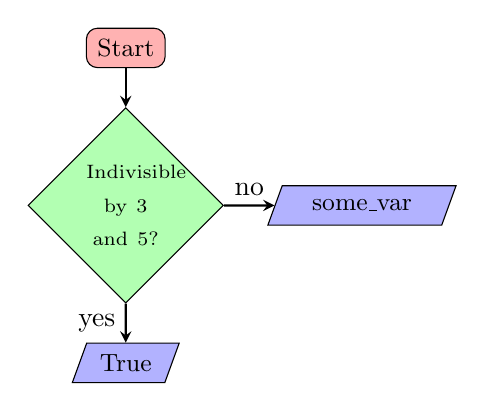
\begin{tikzpicture}[node distance=2cm]
				\node (start) [startstop] {\small{Start}};
				\node (decision) [decision, below of=start, text width=1cm, align=center] {\scriptsize{Indivisible by 3 and 5?}};
				\node (out1) [io, below of=decision] {\small{True}};
				\node (out2) [io, right of=decision, xshift=1cm] {\small{some\_var}};
				\draw [arrow] (start) -- (decision);
				\draw [arrow] (decision) -- node[anchor=east] {yes} (out1);
				\draw [arrow] (decision) -- node[anchor=south] {no} (out2);
			\end{tikzpicture}
		\end{column}
	\end{columns}
\end{frame}

\end{document}
